\documentclass{article}

\usepackage[margin=1in]{geometry}     %for 1inch margins that play nice with fancyhdr
\usepackage{amsmath,amssymb}          % math and junk
\usepackage{fancyhdr}                 % for a nice running header and footer
\usepackage{lastpage}                 % for nice "X of Y" footer
\usepackage[per-mode=symbol,alsoload=binary,detect-all=true]{siunitx}
                                      % for nice units and junk!
\usepackage{gnuplot-lua-tikz}         % enable tikz plots made from gnuplot
\usepackage{float}                    % [H] option for floats
\usepackage[american]{circuitikz}     % for teh circuit diagrams
\usepackage[hidelinks]{hyperref}                 % get those sweet, sweet, links
\usepackage{framed}                   % for framed titlepage
\usepackage{subfig}

\usetikzlibrary{shapes,arrows}

% unused, but common for other experiments
\usepackage{rotating}                 % for sideways stuff!
%\usepackage{cancel}                   % for `canceling out' parts of equations. fancy!
\usepackage{mdwlist}                  % itemize* and friends
%\usepackage{verbatim}                 % for \verbatiminput command and comment environment
\usepackage[colorinlistoftodos]{todonotes}                % todo's, if used/needed
%\usepackage{multirow}                 % for multi-row spans in tabular environment


% values!
\newcommand{\docAuthor}{Sean Barag}
\newcommand{\docCoAuthor}{None}
\newcommand{\ta}{Yang Gao}
\newcommand{\docTitle}{Introducing Control Logic Functionality}
\newcommand{\courseName}{ECE-L304}
\newcommand{\labNum}{Step 6}
\newcommand{\labSec}{064}
\newcommand{\dueDate}{9 March 2012}
\newcommand{\perfDate}{22 \& 29 February, 7 March 2012}

% paths
\graphicspath{{$HOME/texmf/graphics/}}


% meta-data
\pdfinfo{
	/Title    (\labNum: \docTitle)
	/Author   (\docAuthor)
	/Keywords (\docTitle, \labNum)
}

% for fancy header
\pagestyle{fancy}
\lhead{\courseName\ $|$ \labSec}
\chead{\labNum: \docTitle}
\rhead{\docAuthor}
\cfoot{\thepage\ of \pageref{LastPage}}

% title info
\title{\courseName\ \labNum: \\ \docTitle}
\author{\docAuthor}
\date{}

% shortcuts, cause I'm lazy
\newcommand{\bs}[1]{\boldsymbol{#1}}
\newcommand{\tbf}[1]{\textbf{#1}}
\newcommand{\ttt}[1]{\texttt{#1}}

\begin{document}
% Cover page written by Bryndon Blackburn
% Originally written by Bryndon Blalckburn
\begin{titlepage}
	\begin{center}
		\includegraphics[scale = 0.50]{DrexelLogo.pdf}
	\end{center}

	\large
	\begin{framed}
		\begin{center}
			Electrical and Computer Engineering Dept. \\
			Electrical Engineering Laboratory IV, ECE-L304 \\
		\end{center}
	\end{framed} \vspace{50pt}

	\begin{description}
		\item[Title:]\labNum: \docTitle
		\item[Author:] \docAuthor
		\item[Partner:] \docCoAuthor
		\item[Instructor:] \ta
		\item[Section:] \labSec
		\item[Date Performed:] \perfDate
		\item[Date Due:] \dueDate
		\item[Date Received:]
	\end{description}
\end{titlepage}


% Blank page so two-sided printing leaves the cover page on its own sheet
\thispagestyle{empty}
\newpage
\mbox{}

\maketitle
\setcounter{page}{1} % fixes page numbering issues caused by cover sheet
\tableofcontents % this helps
%\newpage
%\listoffigures   % there's over 9000 figures

\newpage % I want the actual content to be at the top of a new page

\section{Introduction}
The entirety of ECE-L304 is devoted to the design, construction, and debugging
of a digital voice recorder.  By providing students with an opportunity to
complete a project of larger scale than anything they have previously
attempted, the course offers its students valuable skills and experience with a
long-term engineering project.

As the system uses digital storage in the form of a RAM chip, it is necessary
to convert all input audio from its native analog form to a digital
representation.  Similarly, the stored digital representation must be converted
back to an analog signal so that it can be correctly rendered by a speaker.
These conversions are performed by an analog to digital converter (ADC) and a
digital to analog converter (DAC), resepectively.
%
In order to ease the design process, students first complete a simple ADC and
DAC simulation.  This helps to remind students of the operating properties and
behaviors of the two converters, as well as providing a schematic similar to
the one required in the final design.

\section{Address Generator}

Students used two~74LS590 8-bit counters to generate the sixteen
least-significant bits of the address generator, as instructed by the lab
manual.  By wiring the most significant bit of one IC into the clock of the
second IC, the two counters will respectively produce the lower byte and higher
byte of the aforementioned sixteen bits.  A similar technique was used to
generate the most significant bit.  By using bit 15 (zero-indexed) as the clock
for a JK flip-flop, bit 16 of the address generator was produced with an
accurate timing.  Figure~\ref{f:add_gen} shows bits 15 and 16 functioning
properly.
%
\begin{figure}[H]
\centering
	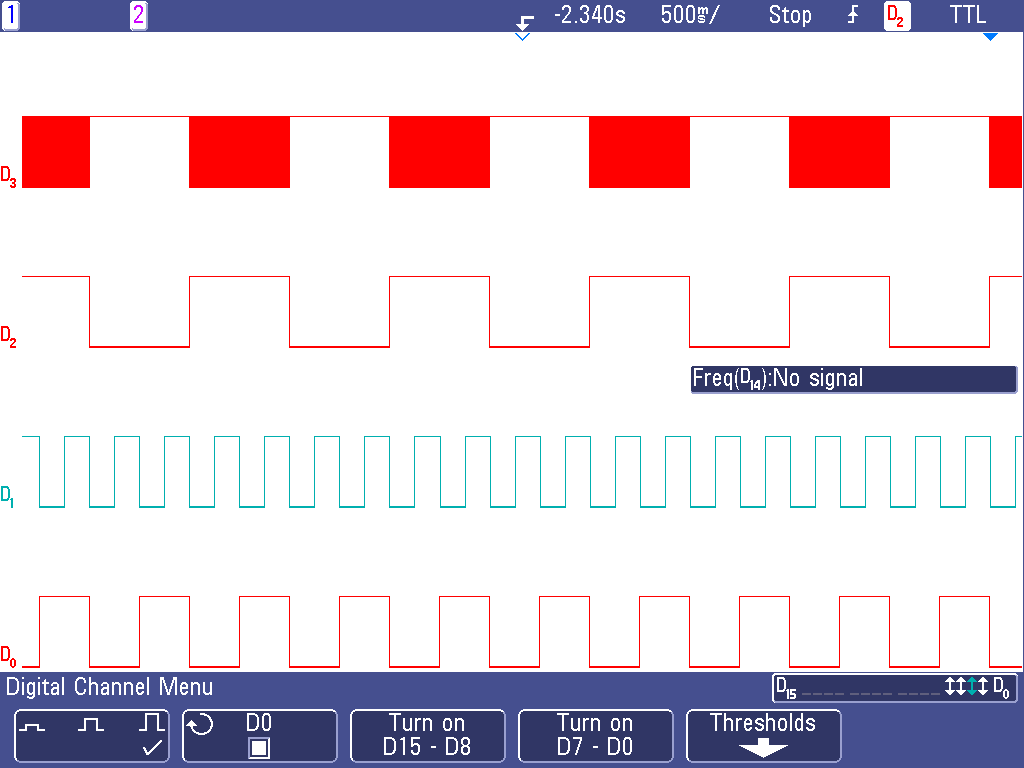
\includegraphics[width=.8\textwidth]{img/shot/add_gen.png}
	\parbox{.8\textwidth}{
	\caption[Functioning Address Generator]{Oscilloscope screenshot of the
	functioning address generator. Note that \ttt{D1} and \ttt{D0} represent
	zero-indexed bits 15 and 16.  Note also that \ttt{D2} and \ttt{D3}
	represent the \ttt{OE} and \ttt{WE} pins.}
	\label{f:add_gen}}
\end{figure}

\section{Clock Delay}

While the clock signal for this system is accurate, students must force the
\ttt{OE} and \ttt{WE} pins to lag slightly behind the generation of individual
memory addresses.  This ensures that the memory address is correct and prevents
the memory address from changing during any single read or write operation.

The actual length of the delay is not critical, but it must be consistent
between clock cycles.  As such, the lab instructors provided a working method
with which the clock signal could be delayed.  By passing the clock through two
series boolean \ttt{AND} gates with the two input pins on each tied together, a
slight delay is introduced into the signal.  Figure~\ref{f:clock} shows such an
effect.
%
\begin{figure}[H]
\centering
	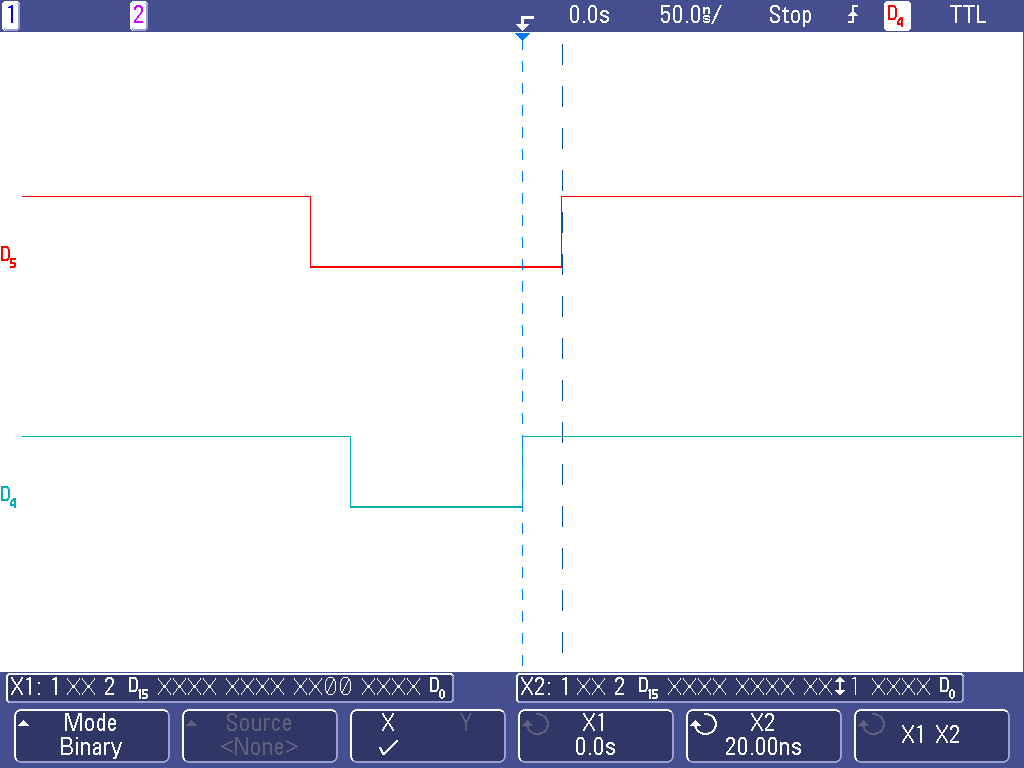
\includegraphics[width=.8\textwidth]{img/shot/and_delay.png}
	\parbox{.8\textwidth}{
	\caption[AND Gate Clock Delay]{Screenshot showing the effects of passing
	the clock signal through two \ttt{AND} gates.  Note that the lower signal
	was measured before entering the \ttt{AND} gates, whereas the upper signal
	was measured at the output of the second gate.  The delay, as measured by
	the oscilloscope, was~\SI{20}{\nano\second}.}
	\label{f:clock}}
\end{figure}
%
Figure~\ref{f:clock} shows the results of delaying the clock signal with two
\ttt{AND} gates from a 74LS08 quad \ttt{AND} IC.  The oscilloscope measured the
delay to be~\SI{20}{\nano\second} --- long enough to ensure that the generated
address has settled, but not so long that it causes the system to become
unstable.

\section{Conclusions}

In conclusion, students simulated a fully functional RAM system in which data
was both stored to and retrieved from the~\SI{64}{kb} RAM chip.   Both the
rudimentary and complex systems exhibited the correct timing behavior, and
reproduced the input data accurately.  While the output of the 8-bit system in
part two showed some anomalies, they are acceptable for the purposes of a basic
voice recorder.  After tuning the complex design so that the anomalies were of
a safe voltage, both systems are ready to be implemented in hardware.


\newpage
\appendix
\section{Used Parts}

By this point in the construction process, the list of used parts has increased
substantially.  A revised list is included in Table~\ref{t:parts}.
%
\begin{table}[H]
	\centering
	\begin{tabular}{|c|c|c|}
		\hline
		\tbf{Part} & \tbf{Description} & \tbf{Quantity} \\ \hline
			74LS590 & 8-bit counter & 2               \\ \hline
			74LS112 & JK Flip-flop (dual package) & 1 \\ \hline
			74LS08  & AND gate (quad package) & 1     \\ \hline
			74LS04  & Inverter (hex package)  & 1     \\ \hline
			LM555   & 555 Timer & 1                   \\ \hline
			ADC0804 & Analog to digital converter & 1 \\ \hline
			DAC0808 & Digital to analog converter & 1 \\ \hline
			$\mu$PD431000A & \SI{1}{\mega\bit} Static RAM & 1 \\ \hline


			Resistor & \SI{1.8}{\kilo\ohm} & 1        \\ \hline
			Resistor & \SI{5}{\kilo\ohm} & 3          \\ \hline
			Resistor & \SI{10}{\kilo\ohm} & 1         \\ \hline
			Resistor & \SI{15}{\kilo\ohm} & 1         \\ \hline
			Capacitor & \SI{151}{\pico\farad} & 1     \\ \hline
			Capacitor & \SI{10}{\nano\farad}  & 1     \\ \hline
	\end{tabular}
	\parbox{.8\textwidth}{
	\caption[Parts List]{ List of parts used in the construction of the voice recorder. }
	\label{t:parts}}
\end{table}

\section{License}

Copyright \copyright\ 2011, Sean Barag.  All rights reserved.

Redistribution and use in source and binary forms, with or without
modification, are permitted provided that the following conditions are met:
\begin{itemize}
\item Redistributions of source code must retain the above copyright notice, this
  list of conditions and the following disclaimer.
\item Redistributions in binary form must reproduce the above copyright notice, this
  list of conditions and the following disclaimer in the documentation and/or
  other materials provided with the distribution.
\item Neither the name of the owner nor the names of its contributors may be
  used to endorse or promote products derived from this software without specific
  prior written permission.
\end{itemize}

THIS SOFTWARE IS PROVIDED BY THE COPYRIGHT HOLDERS AND CONTRIBUTORS ``AS IS'' AND
ANY EXPRESS OR IMPLIED WARRANTIES, INCLUDING, BUT NOT LIMITED TO, THE IMPLIED
WARRANTIES OF MERCHANTABILITY AND FITNESS FOR A PARTICULAR PURPOSE ARE
DISCLAIMED. IN NO EVENT SHALL THE COPYRIGHT HOLDER OR CONTRIBUTORS BE LIABLE
FOR ANY DIRECT, INDIRECT, INCIDENTAL, SPECIAL, EXEMPLARY, OR CONSEQUENTIAL
DAMAGES (INCLUDING, BUT NOT LIMITED TO, PROCUREMENT OF SUBSTITUTE GOODS OR
SERVICES; LOSS OF USE, DATA, OR PROFITS; OR BUSINESS INTERRUPTION) HOWEVER
CAUSED AND ON ANY THEORY OF LIABILITY, WHETHER IN CONTRACT, STRICT LIABILITY,
OR TORT (INCLUDING NEGLIGENCE OR OTHERWISE) ARISING IN ANY WAY OUT OF THE USE
OF THIS SOFTWARE, EVEN IF ADVISED OF THE POSSIBILITY OF SUCH DAMAGE.\\

Source code for this document is available at \texttt{http://github.com/sjbarag/}.


\end{document}
